\chapter{Cryptographic primitives}
\label{chpr:crypto_primitives}
In this section we present the cryptographic primitives which are necessary to build a \textit{confidential transaction}.\\
Prior to this, however, we start with a crash dive into some pillars of Elliptic Curve Cryptography (ECC), the focus being just on what can be useful to follow the incoming narration. We refer, instead, to \cite{Sec} or \cite{UnderstandingCrypto} for a more deep approach.\\
Elliptic Curve Cryptography is a public-key cryptosystem built on elliptic curves defined over finite fields and, for our purposes, it is the cryptosystem Bitcoin uses to secure the transactions. It is based on the intractability of the Elliptic Curve Discrete Logarithm Problem (ECDLP), namely the infeasibility of computing the discrete logarithm of a random elliptic curve point with respect to a publicly known base point\footnote{At the base of public-key cryptography there is always the intractability of a particular mathematical problem: \begin{itemize} \item RSA public-key schemes: hardness of factoring large integers. \item DLP-based public-key schemes: hardness of solving the discrete logarithm problem. \item ECDLP-based public-key schemes: hardness of solving the generalized discrete logarithm over an elliptic curve. \end{itemize}}. The benefits over its prior alternatives (in the field of public-key or asymmetric cryptography) come from the possibility of providing the same security level with shorter operands, which is in turn a consequence of the problem being harder to solve. Indeed, it is even the latest solution which has come out among the mentioned alternatives.\\
Referring to the Appendix \ref{app:A} for both the definition of finite field (and how to get to it) and the presentation of the DLP (in its non-elliptic curve formulations) to avoid making this introduction unintentionally cumbersome, we give instead here the definition of \textit{elliptic curve} and we present the known translation of the DLP over elliptic curves (ECDLP).\\ 
The need to introduce elliptic curves is motivated by the necessity of searching a cyclic group where to build the cryptosystem\footnote{see DLP arguments in \ref{DLP} for more details.}; observe, however, that the mere existence of a cyclic group is not sufficient, the problem being to find such one where the DLP is computationally hard to solve. It turns out that elliptic curves are fitted for the purpose and thus the goal becomes to find elliptic curves with a large cyclic group. Later in this section, a theorem will support the suitability of elliptic curves in providing such a result, thus explaining their fundamental role in the discussion.\\
As remarked within the Appendix \ref{app:A}, for cryptographic use, the focus is just on elliptic curves defined over a finite field (in particular we consider $K = \mathbb{F}_p$, the finite field with p elements) rather than over generic fields (the set $\mathbb{R}$ being an example).
\begin{mydef}
    The elliptic curve over $\mathbb{F}_p$\footnote{which we denote by $E(\mathbb{F}_p)$.} is the set of all pairs $(x,y) \in \mathbb{F}_p$ such that $\{(x,y) \in \mathbb{F}_p \times \mathbb{F}_p: y^2 = x^3 + ax+b \mod p\} \cup \{\infty\}$ with $a,b \in \mathbb{F}_p$ and such that the consistency condition $4 a^3+27b^2 \neq 0 \mod{p}$ holds true.
\end{mydef}
\label{def_EC}
\noindent
The problem now becomes both identifying the group elements and defining a group operation with these elements. Group elements are nothing else than the points fulfilling the curve equation in \ref{def_EC}, the definition of the group operation is not presented here, for the details we refer to \cite{UnderstandingCrypto}.\\
The only point we want to stress is the meaning of $\{\infty \}$ in definition \ref{def_EC}:
\begin{myrem}
    $\{\infty \}$ is the so called infinity point and turns out to be the identity element of the group defined by the points over the elliptic curve together with its group operation.
\end{myrem}
\noindent
At this point, it is possible to state the following theorem, which eventually closes the circle by explaining the reason why it is possible to build a DLP with elliptic curves.
\begin{mytheorem}
    The points on an elliptic curve, together with the infinity point $\{\infty \}$ (other than defining a group by themselves once the group operation is defined) have cyclic subgroups. Moreover, under certain conditions (merely if the group order is prime) all points on an elliptic curve form a cyclic group.
\end{mytheorem}
\begin{myrem}
    By specializing the notation seen in the Appendix \ref{app:A} to the EC case, we denote by $G$ the generator of a cyclic (sub)group defined over an elliptic curve (being an element of the (sub)group itself, it is nothing else than a point on the curve). Thus, starting from $G$ it is possible to explore the entire (sub)group (thus recovering all the (sub)group points) by repeatedly applying the group operation to $G$.
\end{myrem}
\begin{myrem}
    If the EC (sub)group has order $m$, the application of the EC group operation $m$ times gives back the identity element of the EC group.
\end{myrem}
\begin{myrem}
    If the EC group order n is prime, any point of the curve is a generator $G$. This basically comes from \ref{thm::prime_order_all_gen}.
\end{myrem}
\noindent
With this theoretic framework at our disposal, we can conclude the introduction to this chapter by presenting the ECDLP.
\begin{mydef}
    Given the elliptic curve $E(\mathbb{F}_p)$ with generator $G$, consider another element of the curve, $Q$. The ECDLP is finding the integer $q, 1 \leq q \leq \#E(\mathbb{F}_p)$, such that $\underbrace{G+G+\dots+G}_{q \quad times}$=$qG$=$Q$.
\end{mydef}
\noindent
For what concerns notation, in ECC $q$ is the \textit{private key}, which is an integer, while $Q$ is the \textit{public key}, a point on the curve with coordinates $(x_Q, y_Q)$.

\section{Commitment schemes}
\subsection{Additively homomorphic commitment}
\subsection{Pedersen commitment}
\section{Zero-Knowledge Proofs of Knowledge}
\section{Ring signatures}
\section{ECDH}
The elliptic curve Diffie-Hellman primitive is a cryptographic primitive which is at the basis of the ECDH Key Exchange scheme.\\
In turn, the elliptic curve Diffie-Hellman Key Exchange (ECDH) is a key agreement scheme based on ECC, thus relying on the hardness of the ECDLP. It is the EC counterpart of the well known\footnote{in cryptography at least.} Diffie-Hellman Key Exchange (DHKE) protocol. In this section we just present the scheme for the elliptic curve version.\\
It allows two entities, both endowed with an elliptic curve private-public key pair, to engage in a key agreement scheme and establish a shared secret over an insecure channel. The shared secret can then be both used directly as key or as seed to derive other key(s), for instance (but it is just a possibility) via a deterministic generation procedure like RFC6979 (see \cite{rfc6979}).
\subsection{ECDH primitive}
The primitive is built in such a way that both the parties by means of one of their own private key and one of the public key of the other party can recover, autonomously, the same (shared) secret.\\
Here how's the primitive built. Suppose Alice and Bob want to establish a shared secret. The primitive is run autonomously by both and takes as input valid elliptic curve domain parameters $T$\footnote{$T$ = $(p, a, b, G, n, h)$; $p$ specifies the prime finite field $\mathbb{F}_p$; $a,b \in \mathbb{F}_p$ are the coefficients of the elliptic curve equation; $G \in E(\mathbb{F}_p)$ is the elliptic curve generator point; $n$ is the order of $G$, that coincides with the number of points of the cyclic subgroup generated by $G$; $h = \#E(\mathbb{F}_p)/\ n$ is the so called cofactor.}, a private key owned by who is running the procedure ($q_A$ for Alice, $q_B$ for Bob) and the public key corresponding to the other party private key (Alice takes $Q_B$=$q_BG$ as input, Bob takes $Q_A$=$q_AG$ as input\footnote{though, Alice does not obviously know $q_B$, nor Bob $q_A$.}). The output is a shared secret field element $z$ or the string ``invalid" otherwise.\\
The algorithm below refers to the generation of the shared secret from Alice. The same can be done for Bob, by carefully exchanging the roles of the parameters.
\begin{algorithm}
	\caption{ECDH}
	\label{alg:ECDH}
	\begin{algorithmic}[1]
		\Procedure{ecdh}{$T, \ q_A, \ Q_B$}
		\State $S = (x_S,y_S) \gets q_AQ_B$
		\State assert $S \neq \{\infty\}$
		\If {$S = \{\infty\}$}
		\State \textbf{return} ``invalid"
		\EndIf 
		\State \textbf{return} $z \gets x_S \mod{n}$ 
		\EndProcedure
	\end{algorithmic}
\end{algorithm}\\
It turns out to be straightforward to prove that the shared secret computed by both parties is the same. Alice: $q_AQ_B = q_A(q_BG)$; Bob: $q_BQ_A = q_B(q_AG)$ $\rightarrow$ by associativity of the group operation (point addition), the result holds and both compute $S=q_Aq_BG$.
\subsection{ECDH Key Exchange protocol}
According to notation in \cite{Sec}, the key exchange protocol involves a setup phase, a key deployment procedure and a key agreement operation (which actually exploits the ECDH primitive). 
Being constructed on elliptic curves, it is beforehand necessary to agree on the choice of the domain parameters and in particular
\\ \ \\
Here's a simple graphical representation of the key exchange protocol.
\begin{center}
	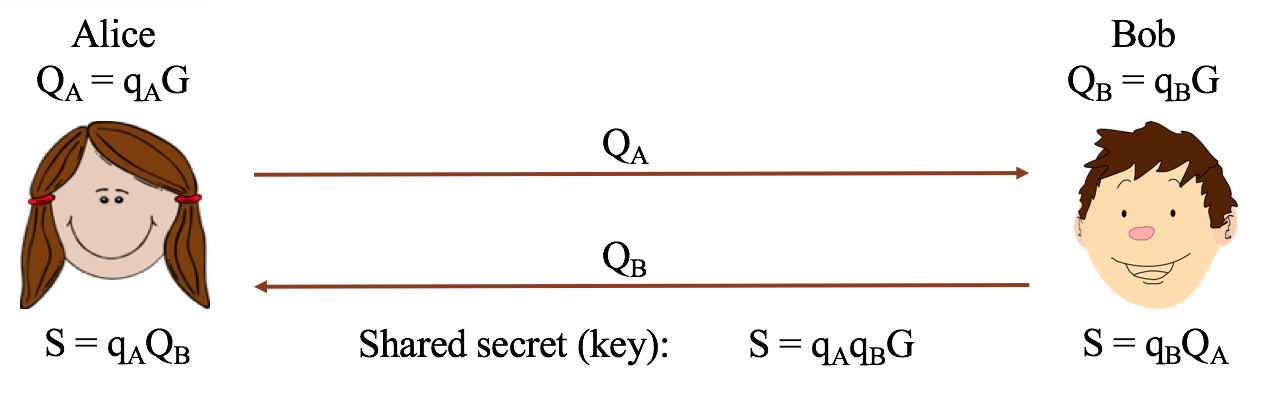
\includegraphics[scale = 0.55]{Images/ECDH.png}
	\captionof{figure}{ECDH key exchange}
	\label{fig:ECDH}
\end{center}
\\ \ \\
Security requirements